\subsection{Play} \label{play}
Play è un framework lightweight, stateless e asincrono per la creazione di applicazioni e servizi Web. È stato costruito utilizzando Scala e Akka e mira a fornire gli strumenti per la realizzazione di applicazioni altamente scalabili con consumo minimo di risorse, ad esempio CPU, memoria, thread \cite{play-framework}.

\medskip

Play incorpora un HTTP Server integrato (quindi non è necessario un server di separato come in molti Web Framework Java), un modello per la realizzazione di applicazioni baste su servizi RESTful e mette a disposizioni strumenti per la gestione di Form, protezione CSRF\footnote{Cross-Site Request Forgery} e meccanismi di instradamento. Per semplificare il suo utilizzo fa largo uso del pattern Model-View-Controller, comune e facilmente utilizzabile, fornendo paradigmi di programmazione concisi e funzionali.

\begin{figure}[H]
\centering
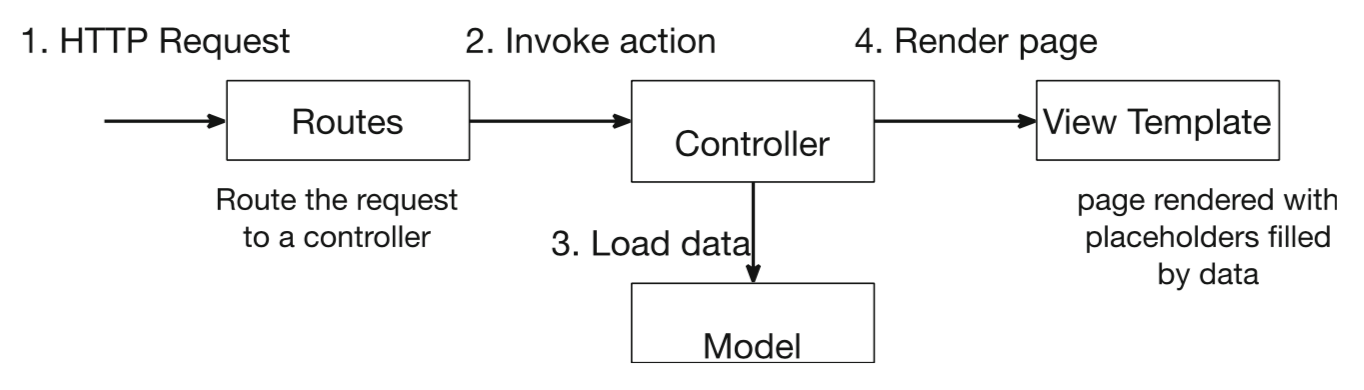
\includegraphics[width=\textwidth]{figures/Play_structure.png}
\caption{Struttura MVC di un'applicazione realizzata con Play \cite{play_framework_book}}
\end{figure}

Lo stack nelle Web Application nel mondo Java Enterprise è basato su una tecnologia che si è evoluta nel corso degli anni e richiede diversi elementi (strati) per funzionare. E' molto probabile che le molteplici tecnologie che comprendono questo stack rendano anche l'implementazione di semplici applicazioni problematica e soggetta a errori poiché ogni tecnologia deve essere integrata con successo con la successiva, spesso basandosi su file di configurazione o convenzioni standard \cite{play_framework_book}.

\begin{figure}[H]
\centering
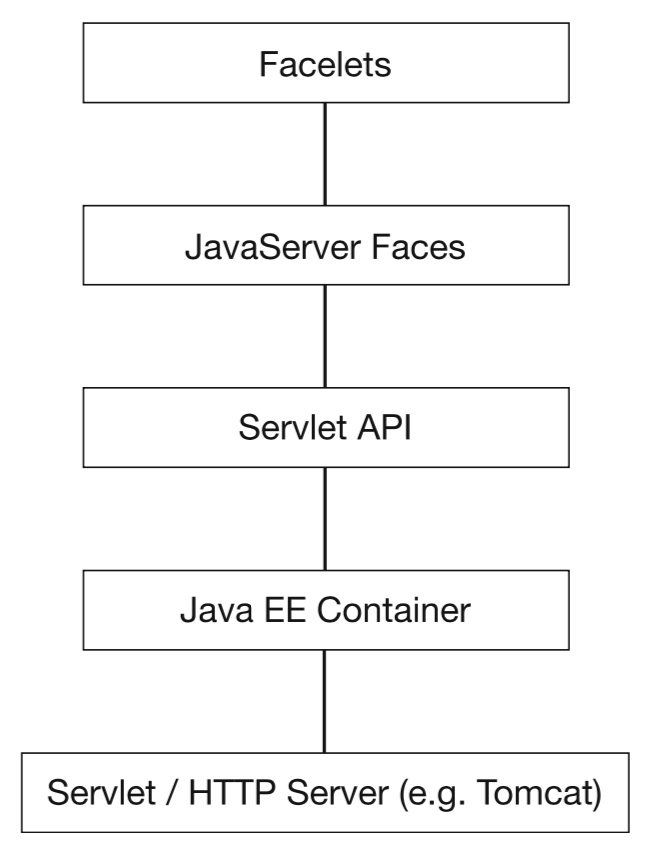
\includegraphics[width=5cm]{figures/Java_EE_layered_architecture.png}
\caption{Architettura a strati JavaEE \cite{play_framework_book}}
\label{Java_EE_layered_architecture}
\end{figure}

Il framework Play è stato progettato per diminuire lo stack (Figura \ref{Java_EE_layered_architecture})  richiedendo l'utilizzo di un solo server HTTP per funzionare.

\begin{figure}[H]
\centering
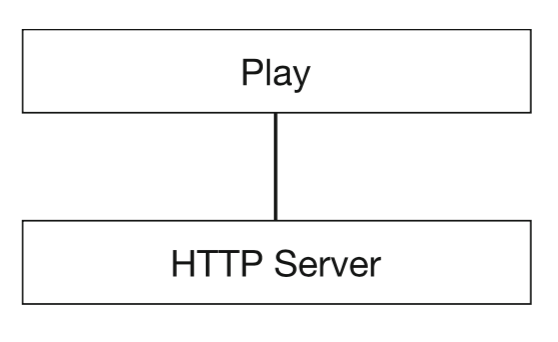
\includegraphics[width=5cm]{figures/Play_layered_architecture.png}
\caption{Architettura a strati Play framework \cite{play_framework_book}}
\label{Play_layered_architecture}
\end{figure}

Lo strato Play (Figura \ref{Play_layered_architecture}) è formato da una serie di componenti che includono:
\begin{itemize}
    \item HTTP Server: componente che riceve la richiesta HTTP da un client e restituisce un risultato basato sulle informazioni fornite nella richiesta;
    \item Router: determina dove instradare la richiesta, pertanto fornisce un file di configurazione dei percorsi disponibili nell'applicativo;
    \item Sistema di templating HTML dinamico: Utilizza pagine standard in HTML e le popola con dati generati dinamicamente dall'applicazione;
    \item Console integrata: Per semplificare l'utilizzo di Play, viene fornita una suite di strumenti che possono essere utilizzati per creare, aggiornare e distribuire l'applicazione Play. Questi strumenti sono accessibili e gestiti dalla console;
    \item Persistent framework: Funzionalità utili per accesso a database.
\end{itemize}
\subsubsection{Akka - Modello ad attori}

Akka è un toolkit per la creazione di applicazioni altamente distribuite, concorrenti, event-driven, tolleranti ai guasti. Play framework utilizza il modello ad attori presente in Akka, dove l'attore è l'entità principale, per aumentare il livello di astrazione e fornire una piattaforma per la realizzazioni di applicazioni concorrenti e scalabili \cite{akka}.

\medskip

Il modello ad attori (che risale al 1973) si basa sull'idea di avere attori simultanei indipendenti che ricevono e inviano messaggi asincroni e che svolgono un comportamento basato su questi messaggi. Gli attori possono mantenere il proprio stato e comportamento. Tuttavia, idealmente solo i dati immutabili vengono scambiati tra di loro, pertanto ogni attore è indipendente da tutti gli altri ed esegue solo alcuni calcoli o elaborazioni basati su un messaggio ricevuto da esso.

\medskip

L'idea chiave alla base del modello ad attori è che la maggior parte dei problemi come concorrenza, deadlock, corruzione dei dati, derivino dalla condivisione dello stato. Pertanto, nel mondo degli attori non esiste uno stato condiviso (come una coda concorrente produttore-consumatore). Al contrario, i messaggi vengono inviati tra attori e questi messaggi vengono messi in coda in una casella di posta in modo simile ai messaggi di posta elettronica \cite{play_framework_book}.

\begin{figure}[H]
\centering
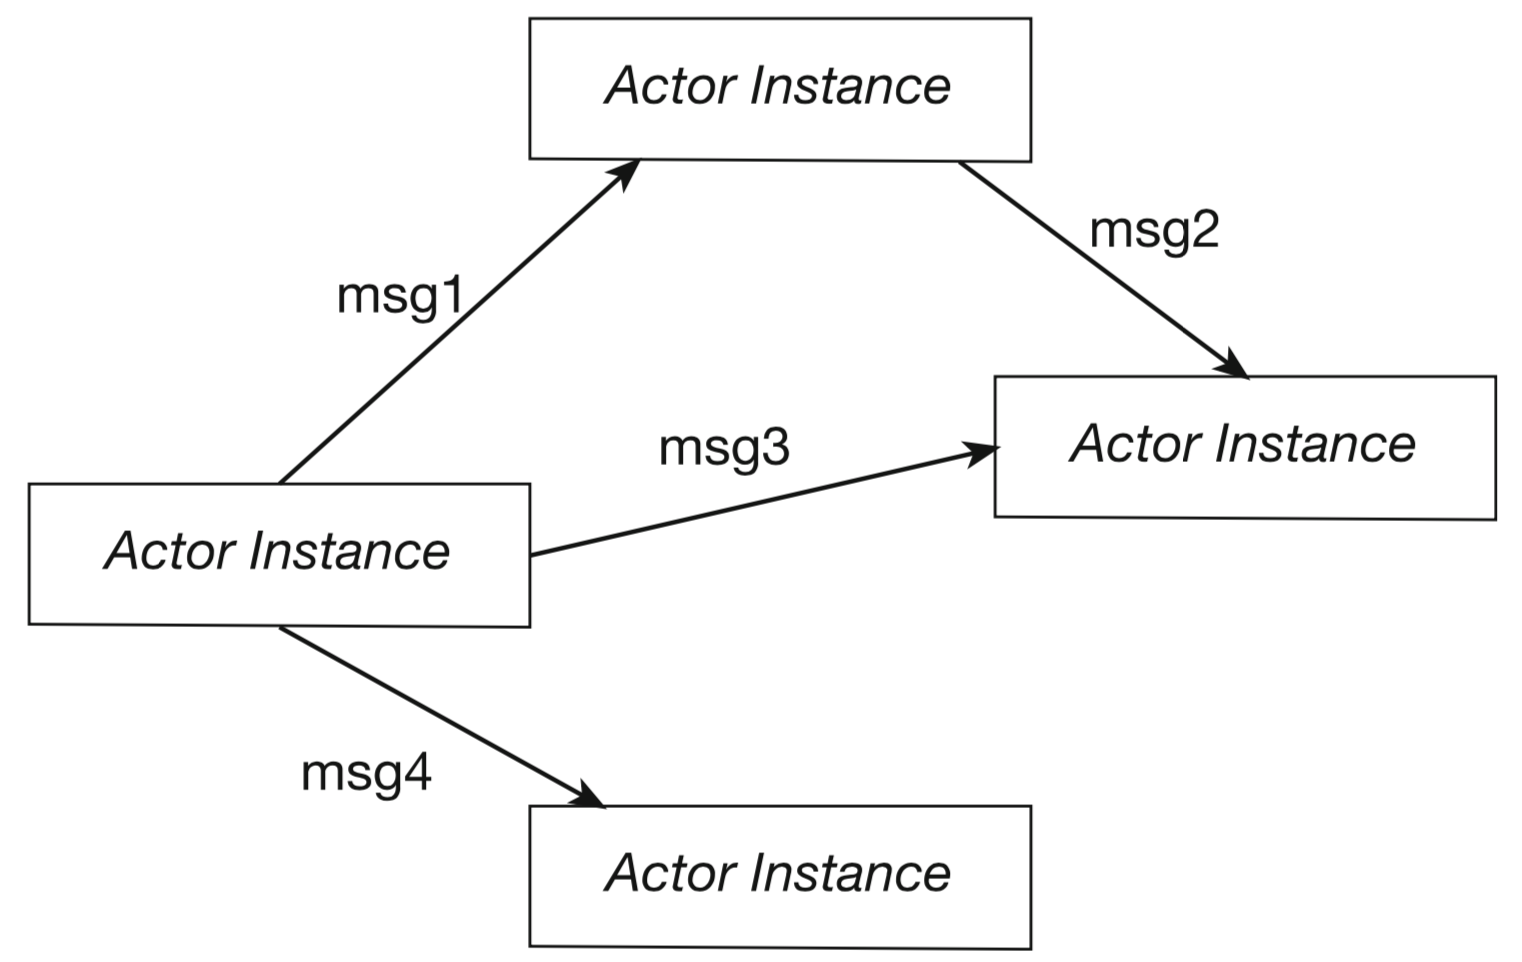
\includegraphics[width=7cm]{figures/Actors_communicating.png}
\caption{Comunicazione tra attori attraverso messaggi asincroni \cite{akka}}
\end{figure}
